\documentclass{article}
\usepackage[utf8]{inputenc}
\usepackage[margin=1in]{geometry}
\usepackage{amsmath}
\DeclareMathOperator{\sech}{sech}
\usepackage{braket}
\usepackage{bbold}
\usepackage{graphicx}
\usepackage{xcolor}
\usepackage{import}
\usepackage{xifthen}
\usepackage{pdfpages}
\usepackage{transparent}

\newcommand{\incfig}[1]{%
    \def\svgwidth{10cm}
    \import{./Figures/}{#1.pdf_tex}
}
\graphicspath{{./Mathematica/}}
\title{Tunnelling Times in Quantum Mechanics}
\author{James Puleston}

\begin{document}

\maketitle

\section{Time in Quantum Mechanics}

\subsection{Time in Classical Mechanics}
In the Hamiltonian formulation of classical mechanics, a system with $n$ degrees of freedom possesses $2n$ independent first-order differential equations in terms of $2n$ independent variables. These variables are the coordinates of the \textit{phase space} of the system, and the $2n$ equations of motion describe the evolution of system in the phase space. $n$ of the independent variables are conventionally chosen to be the generalised coordinates $q_i$ and the other $n$ set to be the conjugate momenta $p_i$, which obey the Poisson bracket relations: \cite{Goldstein}

\begin{equation}
	\{q_i, p_j\}=\delta_{ij} \quad \{q_i, q_j\}=\{p_i,p_j\}=0, \quad i,j=\{1,\dots,n\}
	\label{conjugatevars}
\end{equation}

\noindent The time evolution of the canonical variables is governed by the Hamiltonian $H = H(q_i, p_i)$:

\begin{equation}
	\frac{dq_i}{dt} = \{q_i, H\} \quad \frac{dp_i}{dt} = \{p_i, H\}
	\label{timeevolution}
\end{equation}

\noindent For an infinitesimal variation in time, $\delta t = \delta \tau$, the associated variation in the dynamical variables is:

\begin{equation}
	\delta q_i = \{q_i, H\}\delta\tau \quad \delta p_i = \{p_i, H\}\delta\tau
	\label{timetranslation}
\end{equation}

\noindent $q_i$ and $p_i$ are generalised variables; they are not necessarily positions and momenta, but in the case of a dynamical system comprised of a collection of point particles, the canonical variables are usually the particles' positions $(\boldsymbol{q_i})$ and momenta $(\boldsymbol{p_i})$. 

In classical mechanics, physical systems are embedded in a 4-dimensional continuous space-time background, the points of which are assigned coordinates $(t,x,y,z) = (t, \boldsymbol{x})$.
It is essential that the \textit{definitions} of these two spaces and their associated coordinates are not conflated. In particular we must distinguish the position variable $\boldsymbol{q}$ from the space-time coordinate $\boldsymbol{x}$. The former defines a point in the phase space of the system (when accompanied by its associated momentum $\boldsymbol{p}$) and is a property of a point particle, whereas the latter is the coordinate of a fixed point in the space-time background in which the dynamical system is embedded. Note we can still introduce both sets of quantities in to equations and relate them, as equations (\ref{timeevolution}) and (\ref{timetranslation}) show.

Immediately this raises the question of whether there exists physical systems that possess a dynamical variable that \textit{resembles} the time coordinate of space-time. Such systems are called \textit{clocks}, more precisely defined as physical systems with a dynamical `clock' or `time' variable that behaves similarly to the space-time time coordinate $t$ under time translations. For example, under time translation in which the space-time coordinates transform as:

\begin{equation}
\boldsymbol{x} \rightarrow \boldsymbol{x} \quad t \rightarrow t+\tau
\label{timetranslation2}
\end{equation}

\noindent a \textit{linear} clock variable $\theta$ and its conjugate momentum $\eta$ transform as:

\begin{equation}
	\eta \rightarrow \eta \quad \theta \rightarrow \theta + \tau
	\label{timetranslation3}
\end{equation}

\noindent Comparing with (\ref{timetranslation}) we see in the infinitesimal case of (\ref{timetranslation3}):

\begin{equation}
	\delta\eta=\{\eta, H\}\delta\tau \quad \delta\theta = \{\theta, H\}\delta\tau
	\label{timetranslation4}
\end{equation}

\noindent which implies

\begin{equation}
	\{\eta, H\}=0 \quad \{\theta, H\}=1
	\label{timetranslation5}
\end{equation}

\noindent The equation of motion given by (\ref{timeevolution}), $\frac{d\theta}{dt}=1$ has solution $\theta=t+t_0$.

\subsection{Time in Quantum Mechanics}
\textcolor{red}{3 definitions for time in QM?}
In quantum mechanics the state of a particle is encoded in a vector $\ket{\psi}$ in Hilbert space $\mathcal{H}$. Introducing a 1-dimensional continuum position basis to $\mathcal{H}, \{\ket{q}\}, q \in \mathbb{R}$, the state vector $\ket{\psi}$ can be expanded as the integral:

\begin{equation}
	\ket{\psi} = \int_{\mathbb{R}}dq\psi(q)\ket{q}
\end{equation}

\noindent where $\psi(q)$ is the wave function of the particle. More generally, to describe a system in 3 dimensions requires a wave function $\psi(q_x,q_y,q_z)$. It is important to note that the domain of the wave function is the \textit{configuration space} of the system, $\mathbb{R}^3$, whose coordinates are the generalised coordinates $q_i$ of the system. It is common in elementary quantum mechanics literature for elements of the domain of the wave function to be expressed as $(x,y,z), \text{ i.e. } \psi = \psi(x,y,z)$. This is clearly in notational conflict with the denotation of coordinates of points of the background space-time in which the quantum system resides. 

\textcolor{red}{should I then implement this in the following equations}

Measurable quantities or `observables' are represented by operators on $\mathcal{H}$:

\begin{equation}
	\mathcal{O}: \mathcal{H} \rightarrow \mathcal{H}
\end{equation}

Such operators arise through a procedure called canonical quantisation, which prescribes that \textit{dynamical variables} of the Hamiltonian formalism are promoted to operators on $\mathcal{H}$ and their Poisson bracket relations replaced by commutation relations according to:

\begin{equation}
\{,\} \rightarrow \frac{1}{i\hbar}[,]
\end{equation}

One notable omission in this process is the promotion of the time coordinate $t$ to an operator. Given the emphasis placed on distinguishing between space-time coordinates and dynamical variables, the reason is clear: time t is a \textit{space-time coordinate}, and canonical quantisation prescribes that \textit{dynamical variables} are promoted to operators. However this raises the question of whether a time operator exists in quantum mechanics. Resolution to this problem has been historically hindered by a `proof' offered by Wolfgang Pauli showing that the introduction of a time operator in quantum mechanics is forbidden. It proceeds roughly along the following lines:

\textcolor{red}{Add Pauli proof c.f. Butterfield On Time in Quantum Physics}

Observing that this issue arose from attempts to erroneously quantise the \textit{space-time} coordinate t, the problem becomes void and progress can be made by considering the quantisation of timelike \textit{dynamical variables} of physical systems, namely clocks in analogue with the case in classical mechanics mentioned above. 

\section{Tunnelling Time Candidates}

In this section I survey a number of contenders for calculating the tunnelling time through a barrier. The first of these are theoretical definitions of the time taken to tunnel through a barrier, whereas the remainder are theoretical constructions of quantum clocks that can be used to measure tunnelling times.

\subsection{Tunnelling Through a Quantum Barrier}
\noindent \textcolor{red}{I use Buttiker as the reference barrier, adjusting all other sources accordingly.}

\noindent Consider the case of scattering in one dimension with particles of mass $m$, velocity $v(k) = \frac{\hbar k}{m}$ and kinetic energy $E = \frac{\hbar^2k^2}{2m}$. The particles move along the y-axis and interact with a rectangular barrier:

\begin{equation}
	V = 
	\begin{cases}
	V_0 & -\frac{d}{2}<y<\frac{d}{2}\\
		0 & \text{otherwise}
	\end{cases}
\end{equation}

\begin{figure}[ht]
    \centering
    \incfig{potentialbarrier}
    \caption{The quantum potential barrier}
    \label{fig:potentialbarrier}
\end{figure}

\noindent The wave function is of the form:
\begin{equation}
	\psi = 
	\begin{cases}
		e^{iky} + Ae^{-iky} & y \leq -\frac{d}{2} \\
		Be^{\kappa y} + Ce^{-\kappa y} & -\frac{d}{2} \leq y \leq \frac{d}{2} \\
		De^{iky} & y \geq \frac{d}{2}
	\end{cases}
\end{equation}

\noindent The coefficient of the incident wave is set to one, corresponding to one particle per unit length in the incident beam. Note there is no $e^{-iky}$ term on the right of the barrier, as no particles are reflected after being transmitted through the barrier.

\noindent It is instructive to calculate the wave function coefficients A, B, C, D using the continuity of the wave function and its first derivative at the barrier boundaries. This is a lengthy calculation but the results are used so frequently that it is necessary to include a derivation. The results are stated here and derived below:

\begin{align}
	D &= T^{\frac{1}{2}}e^{i\Delta\phi}e^{-ikd} & A &= R^{\frac{1}{2}}e^{-\frac{i\pi}{2}}e^{i\Delta\phi}e^{-ikd} \nonumber \\
	B &= \frac{\kappa+ik}{2\kappa}e^{\frac{ikd}{2}}e^{\frac{-\kappa d}{2}}D & C &= \frac{\kappa-ik}{2\kappa}e^{\frac{ikd}{2}}e^{\frac{\kappa d}{2}}D \label{cont0}
\end{align}
where $T$ is the transmission probability and $R = 1-T$ is the reflection probability.

\noindent First I introduce a new coordinate system so that the boundaries of our barrier become 0, d. Then, denoting our wave functions before, inside and after the barrier as $\psi_{1}, \psi_{2}, \psi_{3}$ respectively, yields:

\begin{align}
	\psi_{1} &= e^{iky} + Ae^{-iky} & \psi_{1}^{'} &= ike^{iky} - ikAe^{-iky} \\
	\psi_{2} &= Be^{-\kappa y} + Ce^{\kappa y} & \psi_{2}^{'} &= -\kappa Be^{-\kappa y} + \kappa Ce^{\kappa y} \\
	\psi_{3} &= De^{iky} & \psi_{3}^{'} &= ikDe^{iky}
\end{align}

\noindent Imposing continuity of the wave function and its first derivative at the barrier boundaries:
\begin{align}
	\psi_{1}(0) = \psi_{2}(0) &\implies 1+A = B+C \label{cont1}\\
	\psi_{1}^{'}(0) = \psi_{2}^{'}(0) &\implies ik - ikA = -\kappa B + \kappa C \label{cont2}\\
	\psi_{2}(d) = \psi_{3}(d) &\implies Be^{-\kappa d} + Ce^{\kappa d} = De^{ikd} \label{cont3}\\
	\psi_{2}^{'}(d) = \psi_{3}^{'}(d) &\implies -\kappa Be^{-\kappa d} + \kappa Ce^{\kappa d} = ikD e^{ikd} \label{cont4}
\end{align}

\begin{align}
	ik(\ref{cont1})+(\ref{cont2}) &\implies 2ik = B(ik-\kappa)+C(ik+\kappa) \label{cont5}\\
	ik(\ref{cont1})-(\ref{cont2}) &\implies 2ikA = B(ik+\kappa)+C(ik-\kappa) \label{cont6}\\
	\kappa(\ref{cont3})-(\ref{cont4}) &\implies 2\kappa Be^{\kappa d} = De^{ikd}(\kappa-ik) \label{cont7}\\
	\kappa(\ref{cont3})+(\ref{cont4}) &\implies 2\kappa Ce^{\kappa d} = De^{ikd}(\kappa+ik) \label{cont8}
\end{align}

\noindent Inserting equations (\ref{cont7}) and (\ref{cont8}) into equation (\ref{cont5}) one arrives at:

\begin{align}
	2ik &= -\frac{(ik-\kappa)^2}{2\kappa}De^{(ik+\kappa)d}+\frac{(ik+\kappa)^2}{2p}De^{(ik-\kappa)d} \label{cont9} \\
	\implies 4\kappa ike^{-ikd} &= D[(k^2-\kappa^2)(e^{\kappa d}-e^{-\kappa d})+2ik\kappa(e^{\kappa d}+e^{-\kappa d})] \label{cont10}\\
				     &= D[2(k^2-\kappa^2)\sinh{\kappa d}+4ik\kappa \cosh{\kappa d}] \label{cont11}
\end{align}

\noindent Hence one arrives at the first result, the transmission probability $T = |D|^2$:
\begin{equation}
	T = [1+\frac{(k^2+\kappa^2)^2\sinh^2{\kappa d}}{4k^2\kappa^2}]^{-1}
	\label{transmissionprobability}
\end{equation}

\noindent and by writing $D$ in polar form $D = |D|e^{i\theta}$, the phase change across the barrier:

\begin{align}
	D &\propto 4k^2\kappa^2 \cosh{\kappa d}+i2k\kappa(k^2-\kappa^2)\sinh{\kappa d} \\
	  &\implies \Delta \phi := arg(D) = \arctan\left(\frac{\operatorname{Im}(D)}{\operatorname{Re}(D)}\right) = \arctan\left(\frac{(k^2-\kappa^2)}{2k\kappa}\tanh{\kappa d}\right) \label{phasechange}
\end{align}

\noindent Rearranging (\ref{cont11}) for $D$ yields the final result in (\ref{cont0}). The result for A follows along similar lines and results for B and C follow immediately from equations (\ref{cont7}) and (\ref{cont8}). We note that our final results are independent of the coordinate system used (up to scaling by a multiplicative constant) so the result also holds in our other coordinate system.

\subsection{Phase Times}

\noindent Consider a wave packet sharply localised in momentum ($k$) space incident on the barrier. Accounting for time evolution under the time evolution operator $U(t)=e^{-\frac{iEt}{\hbar}}$, the incident wave packet has a peak $y_p(t)$ where the phase of the wave has an extremum when differentiated with respect to $k$:

\begin{equation}
	-\frac{1}{\hbar}\frac{dE}{dk}t+y_p(t)=0
	\label{incidentpeak}
\end{equation}

\noindent This contrasts with the peak of the transmitted wave packet which satisfies:

\begin{equation}
	\frac{d\Delta\phi}{dk}-\frac{1}{\hbar}\frac{dE}{dk}t+y_p(t)-d=0
	\label{transmittedpeak}
\end{equation}

\noindent Solving equations (\ref{incidentpeak}) and (\ref{transmittedpeak}) for $t$ at $y_p(t) = -\frac{d}{2} \text{ and } \frac{d}{2}$ respectively, one finds the traversal time of the peak across the barrier for the transmitted wave to be:

\begin{equation}
	\tau_\phi = \hbar \frac{d\Delta\phi}{dE} = \frac{m}{\hbar k}\frac{d\Delta\phi}{dk}
	\label{buttikerphasetime}
\end{equation}

\noindent An identical result is obtained for a wave packet reflected from the barrier.

\noindent This can be calculated explicitly using equation (\ref{phasechange}):

\begin{align}
	\frac{m}{\hbar k}\frac{d\Delta\phi}{dk}&=\frac{m}{\hbar k}\frac{d}{dk}\left(\arctan{\left[\frac{k^2-\kappa^2}{2k\kappa}\tanh{\kappa d}\right]}\right) \\
					       &=\frac{m}{\hbar k}\frac{1}{\left[\frac{k^2-\kappa^2}{2k\kappa}\tanh{\kappa d}\right]^2+1}\frac{1}{2}\frac{d}{dk}\left(\frac{k^2-\kappa^2}{k\kappa}\tanh{\kappa d}\right) \\ \intertext{The derivative term evaluates to:}
					       &\left[2\kappa^{-1}+\frac{k^2}{\kappa^3}+\frac{\kappa}{k^2}\right]\tanh{\kappa d} + d\left(-\frac{k^2}{\kappa^2}+1\right)\sech^2{\kappa d}\\ \intertext{Hence}
	\frac{m}{\hbar k}\frac{d\Delta\phi}{dk}&=\frac{m}{2\hbar k}\frac{4k^2\kappa^2\sech^2{\kappa d}}{(k^2-\kappa^2)^2\tanh^2{\kappa d}+4k^2\kappa^2}\left\{\left[2\kappa^{-1}+\frac{k^2}{\kappa^3}+\frac{\kappa}{k^2}\right]\sinh{\kappa d}\cosh{\kappa d}-\frac{kd}{\kappa}\left(\frac{k}{\kappa}-\frac{\kappa}{k}\right)\right\}\\
					       &=\frac{2mk\kappa^2}{\hbar}\frac{1}{k_0^4\sinh^2{\kappa d}+4k^2\kappa^2}\left\{\left[2\kappa^{-1}+\frac{k^2}{\kappa^3}+\frac{\kappa}{k^2}\right]\frac{\sinh{2\kappa d}}{2}-\frac{kd}{\kappa}\left(\frac{k}{\kappa}-\frac{\kappa}{k}\right)\right\} \\ \intertext{The term in \{\dots\} is easily shown to be:}
	\{\dots\} &= \frac{k_0^4}{k^2\kappa^3}\frac{\sinh{2\kappa d}}{2}+\frac{d}{\kappa}(\kappa^2-k^2) \\ \intertext{yielding the final result:}
	\tau_\phi &= \frac{m}{\hbar k \kappa}\frac{2k^2\kappa d(\kappa^2-k^2)+k_0^4\sinh{2\kappa d}}{4k^2\kappa^2+k_0^4\sinh^2{\kappa d}} \label{phasedelaytime}
\end{align}

\textcolor{red}{check this, you were tired...}

\noindent B{\"u}ttiker defines this as the phase-delay time of the scattering process. Hauge and St{\o}vneng take an alternative approach and introduce an interval $(x_1, x_2)$ containing the barrier (i.e. $x_1<b,x_2>a$). Using (\ref{incidentpeak}) and (\ref{transmittedpeak}) they define the spatial delay $\delta y_T$ as the change in phase induced by the barrier and corresponding temporal delay $\delta\tau_T$ for the transmitted wave packet:

\begin{equation}
	\delta y_T = \frac{d\Delta\phi}{dk}-d \quad \delta\tau_T=\frac{1}{v(k)} \left[\frac{d\Delta\phi}{dk}-d\right]
	\label{transmittedphaseshift}
\end{equation}

\noindent with analogous definitions for the reflected wave packet:

\begin{equation}
	\delta y_R = d-\frac{d\Delta\phi}{dk} \quad \delta\tau_R=-\frac{1}{v(k)} \left[d-\frac{d\Delta\phi}{dk}\right]
	\label{reflectedphaseshift}
\end{equation}

\noindent They subsequently define the total phase time for transmission:

\begin{equation}
	\tau_T(x_1,x_2;k) = \frac{1}{v(k)}[x_2-x_1+\delta y_T]
\end{equation}

\noindent and similarly the total phase time for reflection:

\begin{equation}
	\tau_R(x_1,x_2;k) = \frac{1}{v(k)}[-2x_1-\delta y_R]
\end{equation}

\noindent where the minus sign before the spatial delay is picked up due to the wave packet travelling in the opposite direction.

\noindent By linearly extrapolating the interval $(x_1,x_2) \rightarrow (-\frac{d}{2},\frac{d}{2})$, one defines the \textit{extrapolated phase times}:

\begin{align}
	\Delta\tau_T(-\frac{d}{2},\frac{d}{2};k) &= \frac{1}{v(k)}[d+\delta y_T] \\
	\Delta\tau_R(-\frac{d}{2},\frac{d}{2};k) &= \frac{1}{v(k)}[d-\delta y_R]
\end{align}

\noindent Substituting in equations (\ref{transmittedphaseshift}) and (\ref{reflectedphaseshift}) to these results recovers (\ref{buttikerphasetime}).

\subsection{Dwell Time}

The dwell time $\tau_D$ is defined as the ratio of the number of particles within the barrier to the incident flux, $\tau_D = \frac{N}{j}$. Clearly this does not distinguish between the scattering channels (reflected or transmitted), so the dwell time is the time a particle spends in the barrier region, averaged over scattering channels.

\noindent One finds for the number of particles in the barrier:

\begin{align}
	N&=\int_{\frac{-d}{2}}^{\frac{d}{2}}|\psi|^2dy \\
	|\psi|^2 &= \frac{T}{4\kappa^2}\left[(\kappa+ik)(\kappa-ik)\left(e^{\kappa(2x-d)}+e^{-\kappa(2x-d)}\right)+(\kappa+ik)^2+(\kappa-ik)^2\right] \\
		 &= \frac{T}{4\kappa^2}\left[(\kappa^2+k^2)\left(e^{\kappa(2x-d)}+e^{-\kappa(2x-d)}\right)+2(\kappa^2-k^2)\right] \\
	\implies N &= \frac{T}{4\kappa^2}\left[\frac{k_0^2}{\kappa}\sinh{2\kappa d}+2(\kappa^2-k^2)d\right] \\ \intertext{using equation (\ref{transmissionprobability}) for $T$:}
		 N &= \frac{k^2}{\kappa}\frac{2\kappa d(\kappa^2-k^2)+k_0^2\sinh{2\kappa d}}{4k^2\kappa^2+k_0^4\sinh^2{\kappa d}}\\ \intertext{and for the incident flux with $\psi = e^{iky}$:
}
	j &= -\frac{i\hbar}{2m}\left(\psi^{*}\frac{\partial\psi}{\partial y}-\psi \frac{\partial \psi^{*}}{\partial y}\right) \\ 
	  &= -\frac{i\hbar}{2m}(2ik) = \frac{\hbar k}{m} = v(k) \\ \intertext{such that:}
	\tau_D &= \frac{1}{v(k)}\frac{k^2}{\kappa}\frac{2\kappa d(\kappa^2-k^2)+k_0^2\sinh{2\kappa d}}{4k^2\kappa^2+k_0^4\sinh^2{\kappa d}}
	\label{dwelltime}
\end{align}

\noindent The phase times $\tau_T \text{ and } \tau_R$ represent conditional averages over mutually exclusive events (a particle cannot both reflect and transmit). The dwell time $\tau_D$ is the average over all scattering channels, and hence the conditional averages must obey the probabilistic rule:

\begin{equation}
	\tau_D = T\tau_T+R\tau_R
\end{equation}

\noindent where $T \text{ and } R = 1-T$ are transmission and reflection probabilities respectively. Comparison of equations (\ref{phasedelaytime}) and (\ref{dwelltime}) show this consistency check is not satisfied. Resolution of this issue comes from noticing that attaching \textit{physical significance} to the time in (\ref{phasedelaytime}) is incorrect, as it requires the assumption that motion outside of the barrier is that of a free particle. This is valid on the transmitted side of the barrier, however during approach to the barrier the incoming wave packet interferes with the reflected wave packet and hence motion can no longer be assumed to be free.

\subsection{Continuous Cyclic Quantum Clock}

In this section I present a theoretical model of a continuous cyclic quantum clock as provided by Hilgevoord. The angular variable $\phi$ plays the role of the clock variable and is represented by the operator $\hat{\Phi}$. An angular momentum operator $\hat{L}$ is also introduced and the two operators in the angular representation are given by:

\begin{equation}
	\hat{\Phi} = \phi \quad \hat{L} = -i \frac{d}{d\phi}
\end{equation}

\noindent as is familiar from the theory of angular momentum in quantum mechanics. These operators act on a Hilbert space of square integrable functions of $\phi$ with domain $[0,2\pi]$ as:

\begin{equation}
	\hat{\Phi} f(\phi) = \phi f(\phi) \quad \hat{L} f(\phi) = -i \frac{d}{d\phi}f(\phi)
\end{equation}

\noindent These operators have eigenvalue equations 

\begin{equation}
	\hat{\Phi}\ket{\phi} = \phi\ket{\phi}, \phi \in [0,2\pi] \quad \hat{L}\ket{m} = m\ket{m}, m = 0, \pm 1, \pm 2,\dots
\end{equation}

\noindent in which the eigenvectors form complete orthonormal sets such that:

\begin{equation}
	\braket{\phi|\phi'} = \delta(\phi-\phi ') \quad \braket{m|m'} = \delta_{mm'}
\end{equation}

\noindent Recalling from the theory of angular momentum in quantum mechanics that the $\hat{L}_z = -i \frac{d}{d\phi}$ operator has eigenfunctions $\propto e^{im\phi}$, $\ket{m}$ has wave function $\braket{\phi|m}= Ae^{im\phi}$ where $A$ is calculated using the normalisation condition to be $(2\pi)^{-\frac{1}{2}}$:

\begin{equation}
	u_m(\phi) := \braket{\phi|m} = (2\pi)^{-\frac{1}{2}}e^{im\phi}
\end{equation}

\noindent As $\{\ket{m}\}$ form a complex set, $\ket{\phi}$ can be expressed as:

\begin{equation}
	\ket{\phi} = (2\pi)^{-\frac{1}{2}}\sum_{m=-\infty}^{\infty}e^{-im\phi}\ket{m}
	\label{phiexpansion}
\end{equation}

\noindent Introducing the Hamiltonian $\hat{H}=\omega \hat{L}$, the time evolution operator $U(t) = e^{-iHt}$ acts as:

\begin{align}
\hat{L}e^{-im\phi}\ket{m} &= e^{-im\phi}\hat{L}\ket{m} \text{ by linearity of } \hat{L} \\
				  &= me^{-im\phi}\ket{m} \\
\implies e^{iHt}\ket{\phi} &= \sum_{n=0}^{\infty}\frac{(-i\omega t)}{n!}^n \hat{L}^n (2\pi)^{-\frac{1}{2}}\sum_{m=-\infty}^{\infty}e^{-im\phi}\ket{m} \\
			   &= (2\pi)^{-\frac{1}{2}}\sum_{n=0}^{\infty}\sum_{m=-\infty}^{\infty} \frac{(-i\omega mt)}{n!}^n e^{-im\phi} \ket{m} \\
				   &= (2\pi)^{-\frac{1}{2}}\sum_{m=-\infty}^{\infty}e^{-i\omega mt}e^{-im\phi}\ket{m} \\
				   &= \ket{\phi+\omega t}
\end{align}

\noindent by setting $\omega = 1, \space \phi$ plays exactly the same role as a time variable $t$.

\subsection{Discrete Cyclic Quantum Clock}
A discrete cyclic quantum clock can be modelled by limiting the sum in equation (\ref{phiexpansion}) to values of \linebreak $m \text{ satisfying } -j \leq m \leq j$, as presented by Peres in [...]. Hence the clock has an odd number $N = 2j+1$ of states represented by wave functions

\begin{equation}
	u_m(\phi) = (2\pi)^{-\frac{1}{2}}e^{im\phi}, m = -j,\dots, j \text{ and } 0 \leq \phi \leq 2\pi
\end{equation}

\noindent One can construct an alternative orthogonal basis for the clock's wave functions

\begin{align}
	v_k(\phi) &= N^{-\frac{1}{2}}\sum_{m=-j}^j e^{-\frac{2\pi ikm}{N}}u_m \label{vkexpansion}\\
		    &= (2\pi N)^{-\frac{1}{2}}\sum_{m=-j}^j [e^{i(\phi-\frac{2\pi k}{N})}]^m \quad \tilde{m} = m+j \\
		    &= (2\pi N)^{-\frac{1}{2}}\sum_{\tilde{m}=0}^{2j} [e^{i(\phi-\frac{2\pi k}{N})}]^{\tilde{m}-j} \\
		    &= (2\pi N)^{-\frac{1}{2}}[e^{i(\phi-\frac{2\pi k}{N})}]^{\frac{1-N}{2}}\sum_{\tilde{m}=0}^{2j}[e^{i(\phi-\frac{2\pi k}{N})}]^{\tilde{m}} \\
		    &= (2\pi N)^{-\frac{1}{2}}[e^{i(\phi-\frac{2\pi k}{N})}]^{\frac{1-N}{2}}\left(\frac{1-(e^{i(\phi-\frac{2\pi k}{N})})^N}{1-e^{i(\phi-\frac{2\pi k}{N})}}\right) \\
		    &= (2\pi N)^{-\frac{1}{2}}\frac{\sin{\frac{N}{2}(\phi-\frac{2\pi k}{N})}}{\sin{\frac{1}{2}(\phi-\frac{2\pi k}{N})}} \text{ for } k = 0,\dots,N-1.
\end{align}

\noindent For large $N$ these functions have a sharp peak at $\phi = \frac{2\pi k}{N}$ which we visualise as pointing to the $k^{th}$ hour with angle uncertainty $\pm \frac{\pi}{N}$:

\begin{center}
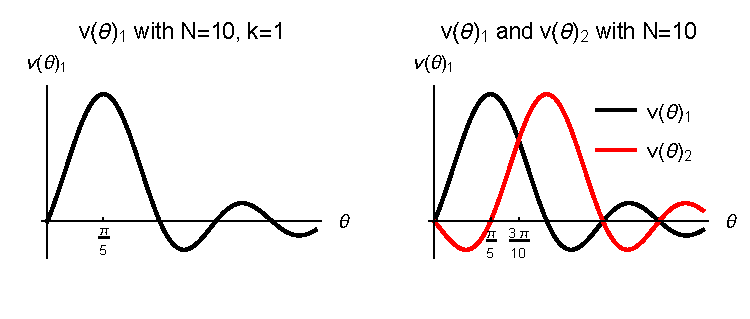
\includegraphics{plot1.pdf}
\end{center}

\noindent One can then define projection operators $P_kv_m=\delta_{km}v_m$ and a clock time operator $T_c = \tau\sum{kP_k}$ where $\tau$ is the resolution of the clock. The eigenvectors of $T_c$ are $v_k$ with eigenvalues $t_k = k\tau, k=0,\dots,N-1$. Hence measuring $T_c$ yields discrete approximations to the true time, just as analog and digital clocks do. 

\noindent The clock's Hamiltonian is:

\begin{equation}
	H_c = \omega J \text{ where } \omega = \frac{2\pi}{N\tau} \text{ and } J=-i\hbar \frac{\partial}{\partial\phi}
	\label{clockhamiltonian}
\end{equation}

\noindent The wave functions $u_m$ are eigenfunctions of the Hamiltonian:

\begin{equation}
	H_cu_m = m\hbar\omega u_m
	\label{clockwavefunctions}
\end{equation}

\noindent whence expanding the time evolution operator as a Taylor series gives:

\begin{align}
	e^{-\frac{iH_ct}{\hbar}}u_m &= e^{-im\omega t}u_m = (2\pi)^{-\frac{1}{2}}e^{im(\theta-\omega t)} \\
	\implies e^{-\frac{iH_c\tau}{\hbar}}v_k &= N^{-\frac{1}{2}}\sum_{m}e^{-\frac{2\pi ikm}{N}}e^{-\frac{2\pi im}{N}}u_m \\
						       &= N^{-\frac{1}{2}}\sum_{m}e^{-2\pi i \frac{m}{N}(k+1)}u_m \\
						       &= v_{k+1}
\end{align}

\subsection{Application: Atomic Decay}
One can apply the construction of the quantum clock to model atomic decay. The atom-clock system has Hamiltonian $H=H_a+P_0H_c$ where $H_a$ is the Hamiltonian of the atom, $H_c$ the Hamiltonian of the clock and $P_0$ the projection operator for the atom's undecayed state, such that the clock stops running when the atom decays. $H_a$ is of the form $H_a=H_0+V$ where $H_0$ has a continuous spectrum $H_0\phi(E) = E\phi(E) \quad E>E_{min}$, plus one discrete eigenstate $\phi_0$ with energy $E_0>E_{min}$. The non vanishing matrix elements of $V$ are denoted $V(E) := \braket{\phi(E)|V|\phi_0}$, which is assumed to be almost constant in $E$ over a large domain on both sides of $E_0$.

\noindent The wave function for the atom can be expressed as:

\begin{equation}
	\psi = a_0\phi_0e^{-\frac{iE_0t}{\hbar}}+\int dE\, a(E)\phi(E)e^{-\frac{iEt}{\hbar}}
\end{equation}

\noindent Application of the Schr{\"o}dinger equation for the atom yields:

\begin{equation}
	i\hbar \dot{a}(E) = V(E)a_0e^{\frac{i(E-E_0)t}{\hbar}}
	\label{aODE}
\end{equation}

\noindent Proof:

\begin{align}
	\ket{\psi} &= a_0\ket{\phi_0}e^{-\frac{iE_0t}{\hbar}}+\int dE\,a(E)\ket{\phi(E)}e^{-\frac{iEt}{\hbar}} \\
	\implies (H_0+V)\ket{\psi} &= a_0E_0\ket{\phi_0}e^{-\frac{iE_0t}{\hbar}}+\int dE\, a(E)E\ket{\phi(E)}e^{-\frac{iEt}{\hbar}} \\ 
				   &+a_0V\ket{\phi_0}e^{-\frac{iE_0t}{\hbar}}+\int dE\, a(E)V\ket{\phi(E)}e^{-\frac{iEt}{\hbar}} \nonumber\\
				   &= i\hbar \frac{d\ket{\psi}}{dt}
\end{align}

\noindent Taking the inner product with $\bra{\phi(E')}$ on both sides and using the orthogonality conditions yields the final result.

\noindent $a_0$ is given by the Weisskopf-Wigner ansatz, $a_0 = e^{-\frac{\gamma t}{\hbar}}$. Substitution into (\ref{aODE}) and taking the limit as $t \rightarrow \infty$ yields:

\begin{equation}
	\lim_{t\to\infty}a(E) = \frac{V(E)}{E-E_0+i\gamma}
\end{equation}

\noindent and 

\begin{equation}
	\lim_{t\to\infty}\psi(t) = \int dE\,\frac{V(E)\phi(E)e^{-\frac{iEt}{\hbar}}}{E-E_0+i\gamma}
\end{equation}

\noindent Normalisation of the wave function implies:

\begin{equation}
	\int dE\,\frac{|V(E)|^2}{(E-E_0)^2+\gamma^2}=1
	\label{atomdecaynormalisation}
\end{equation}

\noindent Utilising the identity:

\begin{equation}
	\delta(E-E_0) = \frac{1}{\pi} \lim_{\gamma\to 0}\frac{\gamma}{(E-E_0)^2+\gamma^2} \approx \frac{\gamma}{\pi} \frac{1}{(E-E_0)^2+\gamma^2}
\end{equation}

\noindent in (\ref{atomdecaynormalisation}) yields $\gamma = \pi|V(E_0)|^2$.

\noindent Coupling the atom to a clock using the clock Hamiltonian in (\ref{clockhamiltonian}):

\begin{equation}
	H = H_a+P_0\omega J
\end{equation}

\noindent and setting the initial state of the clock to $v_0 = \frac{1}{\sqrt{N}}\sum u_n$ as in (\ref{vkexpansion}), $J$ can be replaced by the numerical constant $n\hbar$ by virtue of the eigenvalue equation (\ref{clockwavefunctions}). Note this shifts the energy of the initial state $E_0 \rightarrow E_0 + n\hbar\omega$.

\noindent In the limit of large $t$ the combined state of the atom and clock is:

\begin{equation}
	\psi = N^{-\frac{1}{2}}\sum u_n \int dE \, \frac{V(E)\phi(E)e^{-\frac{iEt}{\hbar}}}{E-E_0-n\hbar\omega+i\gamma}
\end{equation}

\noindent Peres subsequently derives the density matrix representing the state of the clock:

\begin{equation}
	\rho = Tr_a(\ket{\psi}\bra{\psi}) = \frac{1}{N}\sum \frac{\ket{u_n}\bra{u_m}}{1+i\alpha(n-m)}
\end{equation}

\noindent where $Tr_a$ indicates the trace is to be taken over the atom degrees of freedom only, and $\alpha = \frac{\hbar\omega}{2\gamma}$ is the angle through which the pointer turns during an average atom lifetime $\frac{\hbar}{2\gamma}$. From this the probability $\langle P_k \rangle$ of finding the clock stopped at time $t_k = k\tau \stackrel{(\ref{clockhamiltonian})}{=} \frac{2\pi k}{N\omega}$ is given by:

\begin{align}
	Tr(\rho P_k) &= \frac{1}{N}\sum_{m,n} \frac{\braket{v_k|u_n}\braket{u_m|v_k}}{1+i\alpha(n-m)} \\
		     &\stackrel{(\ref{vkexpansion})}{=} \frac{1}{N^2}\sum_{m,n=-j}^j \frac{e^{\frac{2\pi ik(n-m)}{N}}}{1+i\alpha(n-m)}
\end{align}

\noindent The double summation can be evaluated as follows: Let $p=n-m \text{ and } q=n+m$. The summation becomes:

\begin{equation}
	Tr(\rho P_k) = \frac{1}{N^2}\sum_{p=-2j}^{2j}\sum_{q=q_1(p)}^{q_2(p)}\frac{e^{i\theta p}}{1+i\alpha p}
\end{equation}

\noindent where $\theta = \frac{2\pi k}{N}, q_1 \text{ and } q_2$ are bounds that can be determined as follows:

\begin{figure}[ht]
    \centering
    \incfig{doublesumdiagram}
    \caption{Bounds of the double sum in $p,q$ coordinates}
    \label{fig:doublesumdiagram}
\end{figure}

\noindent For fixed $p$, demonstrated by the dashed line in Figure \ref{fig:doublesumdiagram}, the upper and lower bounds can be read off to be:

\begin{equation}
	q_1(p)=-2j+|p| \quad q_2(p)=2j-|p|
\end{equation}

\noindent Next noting that for fixed $p$ of given parity, all $q \in \{q_1(p),\dots,q_2(p)\}$ have the same parity and hence:

\begin{align}
	Tr(\rho P_k) &= \frac{1}{N^2}\sum_{p=-2j}^{2j}\frac{e^{i\theta p}}{1+i\alpha p}\sum_{q=-2j+|p|}^{2j-|p|}1 \\
		     &= \frac{1}{N^2}\sum_{p=-2j}^{2j}\frac{e^{i\theta p}}{1+i\alpha p}\left[\frac{2j-|p|-(-2j+|p|)}{2}+1\right] \\
		     &= \frac{1}{N^2}\sum_{p=-2j}^{2j}\frac{(N-|p|)e^{i\theta p}}{1+i\alpha p} \approx \frac{1}{N}\sum_{p=-2j}^{2j}\frac{e^{i\theta p}}{1+i\alpha p}
\end{align}

\noindent This result can be recognised as the Fourier series expansion of $\frac{2\pi e^{-\frac{\theta}{\alpha}}}{N\alpha\left(1-e^{-\frac{2\pi}{\alpha}}\right)}$, and hence the clocks stop (atoms decay) according to the exponential decay law as expected.

\section{Larmor Precession}

\noindent \textcolor{red}{Work in progress: please ignore for now}

We consider the case of scattering in one dimension with particles of mass $m$, spin $\frac{1}{2}$ and kinetic energy $
E = \frac{\hbar^2k^2}{2m}$. The particles move along the y-axis with spins polarised with the x-axis and interact with a rectangular barrier,

\begin{equation}
	V = 
	\begin{cases}
	V_0 & -\frac{d}{2}<y<\frac{d}{2}\\
		0 & \text{otherwise}
	\end{cases}
\end{equation}

A small magnetic field $\vec{B_{0}}$ points along the z-axis and is confined to the barrier. As particles enter the barrier, the magnetic field induces a Larmor precession with frequency $\omega_{L}=\frac{g \mu B_{0}}{\hbar}$, where $g$ is the gyromagnetic ratio, $\mu$ is the absolute value of the magnetic moment. The polarisations of the transmitted and reflected particles are compared with the polarisation of the incident particles.

Particles initially polarised in the x direction obtain a y and z components when tunnelling through the barrier. We know from the Stern-Gerlach experiment that particles polarised int eh x direction can be represented as combinations of particles with z polarisations, $\ket{x; \pm} = \frac{1}{\sqrt{2}}\ket{z;+} \pm \frac{1}{\sqrt{2}}\ket{z;-}$. Outside the barrier, particles have kinetic energy $E$, independent of their spin. Inside the barrier, the kinetic energy differs by the Zeeman contribution $\pm \frac{\hbar \omega_{L}}{2}$. The wavefunction inside the barrier will contain an exponentially decaying term $Exp(\kappa_{\pm})$, where $\kappa_{\pm} = (k^{2}_{0}-k^{2} \pm \frac{m \omega_L}{\hbar})^{\frac{1}{2}}$, where $\kappa = (k_{0}^2-k^2)^{\frac{1}{2}}$ and the sign indicates spin parallel or antiparallel to the field.  

We can approximate this in the small $\omega_L$ limit as
	\begin{align*}
		\kappa_{\pm} &= \left(k^{2}_{0}-k^{2} \mp \frac{m \omega_{L}}{\hbar}\right)^{\frac{1}{2}}\\	
			     &= \kappa \left(1 \mp \frac{m \omega_{L}}{\hbar \kappa^{2}}\right)^{\frac{1}{2}}\\
			     &\approx \kappa \left(1 \mp \frac{m \omega_{L}}{2\hbar \kappa^{2}}\right)\\
			      &= \kappa \mp \frac{m \omega_{L}}{2\hbar \kappa}
	\end{align*}

Here we examine tunnelling through a barrier in a magnetic field. In this case our Hamiltonian is
\begin{equation}
	H = 
	\begin{cases}
	\left(\frac{p^2}{2m} + V_0\right)\mathbb{1}-\left(\frac{\hbar \omega_L}{2}\right) \sigma_z & |y| \leq \frac{d}{2}\\
	\left(\frac{p^2}{2m}\right)\mathbb{1} & |y| \geq \frac{d}{2}
	\end{cases}
	\end{equation}
where $\mathbb{1}$ is the $2 \times 2$ identity matrix and $\sigma_{x}, \sigma_{y}, \sigma_{z}$ are the Pauli spin matrices.

H acts on spinors
\begin{align}
	\psi &= \begin{pmatrix}
		\psi_{+}(y) \\
		\psi_{-}(y)
		\end{pmatrix}
\end{align}

As usual $|\psi_{\pm}(y)|^{2}dy$ is the probability of finding a particle \textit{upon measurement} with spin $\pm \frac{\hbar}{2}$ in the interval $y, y+dy$. We emphasise the 'upon measurement' here as this is an important point of distinction between the orthodox and pilot-wave interpretations addressed in this essay. The incident beam is polarised in the x direction,
\begin{align}
	\psi &= \frac{1}{\sqrt{2}}
	\begin{pmatrix}
	1\\
	1
	\end{pmatrix}
	e^{i k y}
\end{align}
i.e. $\psi$ is an eigenvector of $S_{x}$

H is diagonal in the spinor basis so we can solve the scattering problem for particles with spin $\frac{\hbar}{2}$ and $-\frac{\hbar}{2}$ separately. 
Our wavefunction is of the form
\begin{equation}
	\psi = 
	\begin{cases}
		A_{\pm}e^{i k y} + B_{\pm}e^{-i k y} & y \leq -\frac{d}{2} \\
		C_{\pm}e^{\kappa_{\pm}y} + D_{\pm}e^{-\kappa_{\pm}y} & -\frac{d}{2} \leq y \leq \frac{d}{2} \\
		F_{\pm}e^{i k y} & y \geq \frac{d}{2}
	\end{cases}
\end{equation}

We will soon set $A_{\pm} = 1$, corresponding to 1 particle per ??, but maintain it for now to aid a future calculation. Note there is no $e^{-i k y}$ term on the right of the barrier, as no particles are reflected. 

The effect of the magnetic field $B_0$ is simply to adjust the height of the barrier, $V_0^{'} = V_0 \pm \frac{\hbar \omega_L}{2}$. Hence we can solve the scattering problem initially assuming no magnetic field, and then adjusting our solution by replacing $\kappa$ in the field-free problem with $\kappa_{\pm}$. Our job now is to calculate the wavefunction coefficients A, B, C, D, F using the continuity of the wavefunction and its first derivative at the boundaries.
This is a lengthy calculation but the results are used so frequently that it is necessary to include a derivation. The results are stated here and derived below:

\begin{align}
	F &= T^{\frac{1}{2}}e^{i\Delta\phi}e^{-ikd} & B &= R^{\frac{1}{2}}e^{-\frac{i\pi}{2}}e^{i\Delta\phi}e^{-ikd} \nonumber \\
	C &= \frac{\kappa+ik}{2\kappa}e^{\frac{ikd}{2}}e^{\frac{-\kappa d}{2}}F & D &= \frac{\kappa-ik}{2\kappa}e^{\frac{ikd}{2}}e^{\frac{\kappa d}{2}}F
\end{align}
where $T$ is t:he transmission probability and $R = 1-T$ is the reflection probability.

First we introduce a new coordinate system so that the boundaries of our barrier become 0, d. Then, denoting our wavefunctions before, inside and after the barrier as $\psi_{1}, \psi_{2}, \psi_{3}$ respectively, we have:

\begin{align}
	\psi_{1} &= Ae^{iky} + Be^{-iky} & \psi_{1}^{'} &= Aike^{iky} - ikBe^{-iky} \\
	\psi_{2} &= Ce^{-\kappa y} + De^{\kappa y} & \psi_{2}^{'} &= -\kappa Ce^{-\kappa y} + \kappa De^{\kappa y} \\
	\psi_{3} &= Fe^{iky} & \psi_{3}^{'} &= ikFe^{iky}
\end{align}

Imposing continuity of the wavefunction and its first derivative at the barrier boundaries:
\begin{align}
	\psi_{1}(0) = \psi_{2}(0) &\implies A+B = C+D \\
	\psi_{1}^{'}(0) = \psi_{2}^{'}(0) &\implies ikA - ikB = -\kappa C + \kappa D \\
	\psi_{2}(d) = \psi_{3}(d) &\implies Ce^{-\kappa d} + De^{\kappa d} = Fe^{ikd} \\
	\psi_{2}^{'}(d) = \psi_{3}^{'}(d) &\implies -\kappa Ce^{-\kappa d} + \kappa De^{\kappa d} = ikF e^{ikd} 
\end{align}

\begin{align}
	ik(\ref{cont1})+(\ref{cont2}) &\implies 2ikA = C(ik-\kappa)+D(ik+\kappa) \\
	ik(\ref{cont1})-(\ref{cont2}) &\implies 2ikB = C(ik+\kappa)+D(ik-\kappa) \\
	\kappa(\ref{cont3})-(\ref{cont4}) &\implies 2\kappa Ce^{\kappa d} = Fe^{ikd}(\kappa-ik)\\
	\kappa(\ref{cont3})+(\ref{cont4}) &\implies 2\kappa De^{\kappa d} = Fe^{ikd}(\kappa+ik) 
\end{align}

Inserting equations (\ref{cont7}) and (\ref{cont8}) into equation (\ref{cont5}) we arrive at:

\begin{align}
	2ikA &= -\frac{(ik-\kappa)^2}{2\kappa}Fe^{(ik+\kappa)d}+\frac{(ik+\kappa)^2}{2p}Fe^{(ik-\kappa)d} \\
	\implies 4\kappa ikAe^{-ikd} &= F[(k^2-\kappa^2)(e^{\kappa d}-e^{-\kappa d})+2ik\kappa(e^{\kappa d}+e^{-\kappa d})] \\
				     &= F[2(k^2-\kappa^2)\sinh{\kappa d}+4ik\kappa \cosh{\kappa d}] 
\end{align}

One arrive at the first result, the transmission probability $T = \frac{|F|^2}{|A|^2}$:
\[
	T = [1+\frac{(k^2+\kappa^2)^2\sinh^2{\kappa d}}{4k^2\kappa^2}]^{-1}
.\] 

and, by writing $D$ in polar form $D = |D|e^{i\theta}$, the phase change across the barrier:
i
\begin{align}
	D &\propto 4k^2\kappa^2 \cosh{\kappa d}e^{-ikd}+i2k\kappa(k^2-\kappa^2)\sinh{\kappa d}e^{-ikd} \\
	  &\implies \Delta \phi := arg(D) = \arctan\left(\frac{\operatorname{Im}(D)}{\operatorname{Re}(D)}\right) = \arctan\left(\frac{(k^2-\kappa^2)}{2k\kappa}\tanh{\kappa d}\right) \\
	  &\implies De^{ikx}\rvert_{x=d}-e^{ikx}\rvert_{x=0} = |D|e^{i\Delta \phi}e^{ik(d-d)}-1 \\
	  \text{and so the phase change} = \Delta \phi
\end{align}

It is clear now why we left the coefficient A explicit, but from now on it will be set to A = 1.

Rearranging (\ref{cont11}) for $F$, we can compare with the final result in (\ref{cont0}) and factorise out $T^\frac{1}{2}$:

\[
	F = T^{\frac{1}{2}}e^{-ikd} \times \frac{(k^2-\kappa^2)i\sinh{\kappa d}+2k\kappa \cosh(\kappa d)}{\sqrt{(k^2+\kappa^2)^2\sinh^{2}{\kappa d}+4k^2\kappa^2}}
\] 
This yields the identification

\begin{align}
	e^{i\Delta\phi} &= \frac{(k^2-\kappa^2)i\sinh{\kappa d}+2k\kappa \cosh{\kappa d}}{\sqrt{(k^2+\kappa^2)\sinh^{2}(\kappa d)+4k^2\kappa^2}} \\
			&= \frac{(k^2-\kappa^2)i\tanh{\kappa d}+2k\kappa}{\sqrt{(k^2-\kappa^2)^2\tanh^2{\kappa d}+4k^2\kappa^2}}
\end{align}

Expanding the left hand side into real and imaginary parts and comparing coefficients we deduce:

\[
	\tan{\Delta\phi} = \frac{(k^2-\kappa^2)\tanh(\kappa d)}{2k\kappa}
\] 

The result for B follows along similar lines and results for C and D follow immediately from equations (\ref{cont7}) and (\ref{cont8}). We note that our final results are independent of the coordinate system used (up to scaling by a multiplicative constant) so the result also holds in our other coordinate system.

\begin{thebibliography}{100}
\bibitem{Goldstein}
Goldstein

\end{thebibliography}
\end{document}
